\section{ULF Parsing}

\begin{figure}
\centering
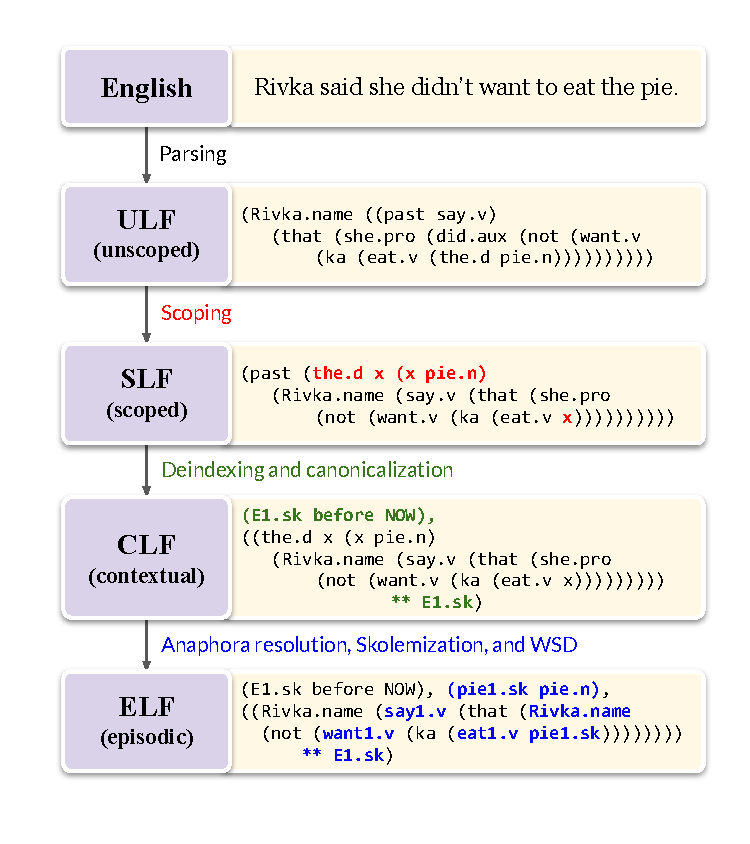
\includegraphics[width=\columnwidth]{CH2_el/el_pipeline.pdf}
\label{fig:el_pipeline}
\caption{The stages of the Episodic Logic parsing pipeline. Solid arrows represent the flow of data through the pipeline, and are labeled with the steps needed to obtain the target forms. The relevant changes are highlighted in each stage's example.}
\end{figure}

\label{subsec:ulf}
Unscoped Logical Form (ULF), an intermediate form of Episodic Logic, formally represents the semantic types and predicate-argument structures of natural language. It is the first, and most developed, step in the ``divide and conquer'' approach to EL parsing illustrated in Figure~\ref{fig:el_pipeline}. In order to obtain ELFs from ULFs, one must, at the very least, perform quantifier scoping, resolve anaphora, deindex the temporal coordinates of events, disambiguate word senses \footnote{Though, as in natural logic, inference is often possible without full word sense disambiguation.}, and \textit{canonicalize} ELFs (minimize ELFs into separate propositions by Skolemizing existentially quantified variables at the top level).

\citet{kim2022corpus} fully describes ULF and the current state of ULF parsing. In this section, we describe our language model-based ULF parser \citep{gibson2022language} and evaluate it against two other ULF parsers: a symbolic, rule-based transduction from constituency parses \citep{kim2021naloma} and a neural cache transition parser \citep{kim2021transition}, ultimately justifying our choice of the rule-based transduction method.

\subsection{Language Model-Based ULF Parsing}
In crafting an EL parsing pipeline, we experimented with using GPT-2, a state-of-the-art language model architecture based on a decoder-only transformer \citep{Radford2019LanguageMA}. Our intuition was that, given ULF's similarity to the syntactic surface form of English, a pre-trained language model might be able to perform well at ULF parsing by casting the problem as one of translation. In this light, we fine-tuned GPT-2 models to perform translation not just of English into ULF (parsing), but of ULF into English (verbalization). This section describes those models and the experiments performed on them.
\subsubsection{Objective}
%Like \citet{gpt-too}, we chose to fine-tune the GPT-2 \citep{Radford2019LanguageMA} language model to perform both of our tasks. Our approach differs slightly in that we did not adapt the default tokenizer to the ULF syntax, nor did we add the \texttt{\textbf{<SEP>}} or \texttt{\textbf{<END>}} tokens to the GPT-2 vocabulary, as modifying the tokenizer did not meaningfully improve performance on either task.
Given a tokenized English sentence $e = e_{1} \cdot e_{2} \cdot \ldots \cdot e_{m}$ and a tokenized s-expression representation of a corresponding ULF $u = u_{1} \cdot u_{2} \cdot \ldots \cdot u_{n}$, we fine-tuned our English-to-ULF GPT2 model for 327 epochs to maximize the joint probability of the concatenated sequences \footnote{The special tokens \texttt{<SEP>} and \texttt{<END>} were included between and after the two concatenated sequences, respectively, for every pair in the dataset.} $e$ and $u$, $P_{\textrm{GPT2}}(u,e) = P_{\textrm{GPT2}}(u|e) \cdot P_{\textrm{GPT2}}(e)$, where:

\vspace{3mm}

$$\mathlarger{P_{\textrm{GPT2}}(u|e) = \prod_{i=1}^{n} P_{\textrm{GPT2}}(u_{i} | e_{1:m},u_{1:i-1})}$$
\vspace{1mm}

$$\mathlarger{P_{\textrm{GPT2}}(e) = \prod_{j=1}^{m} P_{\textrm{GPT2}}(e_{j} | e_{1:j-1})}$$

\vspace{3mm}

The maximization objective for the ULF-to-English verbalization model is obtained by instead decomposing the joint probability $P_{\textrm{GPT2}}(u,e)$ into the similarly defined $P_{\textrm{GPT2}}(e|u)$ and $P_{\textrm{GPT2}}(u)$.

\subsubsection{Dataset}

We used the hand-annotated ULF dataset provided by \citet{kim2021transition}, comprising 1,738 sentences. We split our training (1,378), development (180), and test (180) sentences as prescribed in that paper. The data splitting aims to evenly distribute document-level topics among each subset of the sentences, and to avoid score inflation from linguistic similarity between adjacent sentences.

%For each English-ULF pair in the dataset, we produced fine-tuning data as seen in Figure~\ref{fig:dataset}.
To fine-tune the language model on these pairs, we constructed for each pair a tokenized English sentence $e = e_{1} \cdot e_{2} \cdot \ldots \cdot e_{m}$ and a tokenized s-expression representation of the corresponding ULF $u = u_{1} \cdot u_{2} \cdot \ldots \cdot u_{n}$. We fine-tuned our English-to-ULF and ULF-to-English GPT-2 models to maximize the joint probability of the concatenated sequences. \footnote{The special tokens \texttt{<SEP>} and \texttt{<END>} were included between and after the two concatenated sequences, respectively, for every pair in the dataset.}

To obtain each task's final model, we used the Huggingface transformer library to fine-tune the 774M-parameter \texttt{gpt2-large} model for 327 epochs with a block size of 128.

\subsubsection{Generation}

The trained model yields probability distributions over all tokens for each element in the output sequence ($\hat{e}_{i}$ for generated English and $\hat{u}_{j}$ for generated ULF). We experimented with several decoding methods for obtaining output strings from these probability distributions. As \citet{gpt-too} did, we evaluated generations for both tasks decoded using beam search, greedy sampling, nucleus (top-$p$) sampling.

We additionally evaluated generations decoded using thermal sampling, where, prior to a weighted random token selection, $p_{i,t}$, the probability of each token $t$ at each position $i$, is transformed according to $\tilde{p}_{i,t} = p_{i,t}^{\frac{1}{\tau}}\ /\ \sum_{j} p_{i, t}^{\frac{1}{\tau}}$, controlled by the temperature parameter $\tau$. When $\tau = 0$, thermal sampling is equivalent to greedy sampling.

For the verbalization model, all decoding methods were evaluated with and without the \elsmatch re-scoring described in Section~\ref{subsec:rescoring}; the results are presented in Table~\ref{T3}, and support the choice of the 10-beam, non-rescored decoder for the comparisons to other parsers in Section~\ref{subsec:ulf-eval}. For the parsing model, we used the same choice of decoder.

\vspace{5mm}

\begin{table}[ht]
\centering
\begin{tabular}{l|c|c|c}
\toprule
\multicolumn{1}{c|}{\textbf{Model}}&\multicolumn{1}{c|}{\textbf{BLEU}}&\multicolumn{1}{c|}{\textbf{chrF++}}&\multicolumn{1}{c}{\textbf{METEOR}}\\
% \textbf{CORA}&\textbf{Citeseer}&\textbf{Pubmed}
%\midrule
%Model&Accuracy&Accuracy&Accuracy\\
\midrule
\texttt{Greedy}&0.67&0.81&0.76\\
\texttt{Greedy (els)}&0.67&0.81&0.76\\
\texttt{Beam 10}&\textbf{0.72}&\textbf{0.84}&\textbf{0.80}\\
\texttt{Beam 10 (els)}&\textbf{0.72}&\textbf{0.84}&\textbf{0.80}\\
\texttt{Beam 15}&\textbf{0.72}&\textbf{0.84}&\textbf{0.80}\\
\texttt{Beam 15 (els)}&\textbf{0.72}&\textbf{0.84}&\textbf{0.80}\\
\texttt{Nucleus}&0.68&0.82&0.77\\
\texttt{Nucleus (els)}&0.68&0.82&0.78\\
\texttt{Temp 0.5}&0.69&0.82&0.77\\
\texttt{Temp 0.5 (els)}&0.71&\textbf{0.84}&0.79\\
\texttt{Temp 1.0}&0.67&0.81&0.77\\
\texttt{Temp 1.0 (els)}&0.66&0.81&0.77\\
\bottomrule
\end{tabular}\\[10pt]
\caption{Results for all decoding methods in our ULF-to-English verbalization model, with and without an \elsmatch re-scoring term (\texttt{els}) added to the generated log probability. All scores are out of 1.0.\label{T3}}
\end{table}

\subsubsection{Sample Re-Scoring for Verbalizations}
\label{subsec:rescoring}
In \citep{gpt-too}, the top K generated ULF formulas from the beam search decoder were re-scored by parsing each sentence back into AMR and then computing a cycle consistency score between the parsed and input AMR graphs. They showed that re-scoring based on the ability of an external parser to re-construct the original input from the generated output improved performance.

Likewise, in our ULF-to-English verbalization model, we re-score generated English samples by using an external ULF parser to re-construct the input ULF. In place of a cycle consistency score, we use \elsmatch, which is described in Section~\ref{subsec:ulf-eval}, as a metric for ULF similarity during re-scoring. We did not construct an analogous re-scoring procedure for the English-to-ULF parsing model, as data from the verbalization experiment (Table~\ref{T3}) did not support the use of re-scoring in the reverse direction.
\iffalse
\subsection{Language Model-Based ULF Parsing}
In crafting an EL parsing pipeline, we experimented with using GPT-2, a state-of-the-art language model architecture based on a decoder-only transformer \citep{Radford2019LanguageMA}. Our intuition was that, given ULF's similarity to the syntactic surface form of English, a pre-trained language model might be able to perform well at ULF parsing by casting the problem as one of translation.

To fine-tune the language model, we used the corpus of English sentences paired with hand-annotated ULFs provided by \citet{kim2021transition}. We split our training (1,378), development (180), and test (180) sentences as prescribed in that paper. The data splitting aims to evenly distribute document-level topics among each subset of the sentences, and to avoid score inflation from linguistic similarity between adjacent sentences.

Given a tokenized English sentence $e = e_{1} \cdot e_{2} \cdot \ldots \cdot e_{m}$ and a tokenized s-expression representation of a corresponding ULF $u = u_{1} \cdot u_{2} \cdot \ldots \cdot u_{n}$, we fine-tuned our English-to-ULF GPT2 model for 327 epochs to maximize the joint probability of the concatenated sequences \footnote{The special tokens \texttt{<SEP>} and \texttt{<END>} were included between and after the two concatenated sequences, respectively, for every pair in the dataset.} $e$ and $u$, $P_{\textrm{GPT2}}(u,e) = P_{\textrm{GPT2}}(u|e) \cdot P_{\textrm{GPT2}}(e)$, where:

\vspace{3mm}

$\mathlarger{P_{\textrm{GPT2}}(u|e) = \prod_{i=1}^{n} P_{\textrm{GPT2}}(u_{i} | e_{1:m},u_{1:i-1})}$
\vspace{1mm}

$\mathlarger{P_{\textrm{GPT2}}(e) = \prod_{j=1}^{m} P_{\textrm{GPT2}}(e_{j} | e_{1:j-1})}$

\vspace{3mm}

To generate ULFs from English sentences, the model is prompted with an English sentence and the separator token \texttt{<SEP>}, and stopped after it produces the end token \texttt{<END>}. We choose from the space of possible completions by running a beam search, with 10 beams, for the sequence with the highest cumulative log probability.
\fi

\subsection{ULF Parser Evaluation and Comparison}
\label{subsec:ulf-eval}
We evaluate all ULF parsers in the manner of \citet{kim2021transition}: ULFs are converted into the penman format \citep{kasper-1989-flexible} and evaluated using the \elsmatch \citep{kim2016high} and \sembleu \citep{song-gildea-2019-sembleu} metrics. As another semantic representation, the Abstract Meaning Representation (AMR) \citep{amr}, is convertible to the same penman format, comparisons to two AMR parsers---the sequence-to-sequence graph parser (STOG) \citep{zhang-etal-2019-amr} and the graph-sequence iterative inference parser (GS) \citep{cai-lam-2020-amr}---are also possible, and were evaluated by \citet{kim2021transition}. The results of the evaluation are given in Table~\ref{T2}.

\begin{table}
\centering
\begin{tabular}{c|c|c}
\toprule
\multicolumn{1}{c|}{\textbf{Model}}&\multicolumn{1}{c|}{\sembleu}&\multicolumn{1}{c}{\elsmatch}\\
% \textbf{CORA}&\textbf{Citeseer}&\textbf{Pubmed}
%\midrule
%Model&Accuracy&Accuracy&Accuracy\\
\midrule
\texttt{STOG} \citep{zhang-etal-2019-amr}&0.13&0.34\\
\texttt{GS} \citep{cai-lam-2020-amr}&0.34&0.53\\
\texttt{cache-transition} \citep{kim2021transition}&\textbf{0.47}&0.60\\
\texttt{\textbf{ulf-from-sentences}}&\textbf{0.47}&\textbf{0.65}\\
\texttt{ulf-gpt2}&0.43&0.63\\
\bottomrule
\end{tabular}\\[10pt]
\caption{ULF parsing performance evaluations. All scores are out of 1.0; bolded scores and models are the best. \texttt{ulf-from-sentences} is the rule-based transduction parser mentioned in \citep{kim2021naloma}.}
\label{T2}
\end{table}